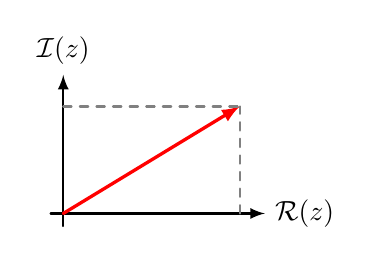
\begin{tikzpicture}
    [>=latex, 
    line cap=round,
    line join=round,
    scale=0.8]

    \draw[->, thick] (-0.2, 0  ) -- (3.2, 0 ) node[right] {$\mathcal{R}(z)$};
    \draw[->, thick] (0,   -0.2) -- (0,  2.2) node[above] {$\mathcal{I}(z)$};
        
    \draw[->, very thick, red] (0, 0) -- (2.8, 1.7);

    % Hilfslinien
    \draw[dashed, thick, gray] (2.8, 0) -- (2.8, 1.7);
    \draw[dashed, thick, gray] (0, 1.7) -- (2.8, 1.7);
\end{tikzpicture}